% Chapter 1

\chapter{Introduction} % Main chapter title

\label{Chapter1} % For referencing the chapter elsewhere, use \ref{Chapter1} 

%----------------------------------------------------------------------------------------

% Define some commands to keep the formatting separated from the content 
\newcommand{\keyword}[1]{\textbf{#1}}
\newcommand{\tabhead}[1]{\textbf{#1}}
\newcommand{\code}[1]{\texttt{#1}}
\newcommand{\file}[1]{\texttt{\bfseries#1}}
\newcommand{\option}[1]{\texttt{\itshape#1}}

%----------------------------------------------------------------------------------------
\section{Graft versus Host Disease}
\subsection{Clinical Background}

Allogeneic hematopoietic stem cell transplant (HSCT) represents the primary treatment for multiple malignant and nonmalignant diseases that would often prove fatal without intervention. However the current efficacy of HST is hampered by the fact that many patients go on to develop Graft-versus-Host Disease (GVHD), a condition that represents the most serious and life threatening complication to arise from this treatment with an overall mortality rate of 15\% ~\autocite{Fur2015, Bla2012}. Prior to HSCT, recipients undergo a conditioning regimen that is not only myelosuppressive to deplete the host immune system and facilitate donor stem cell engraftment, but is also immunosuppressive thus reducing the likelihood of graft rejection ~\autocite{Bla2012}. Indeed it is the toxicity and suppressive effects of this regimen that, by precipitating tissue damage and inflammation in the host, can lead to the development of clinical GVHD. This pre-HSCT conditioning usually takes the form of chemotherapy and is followed by the transfer of a stem cell graft. CD4+ and CD8$\textsuperscript{+}$ T cells are often co-transplanted with the graft and represent the primary immunocompetent population of cells that mediated a beneficial anti-tumour response known as Graft-versus-Leukaemia (GVL) ~\autocite{Pac2013}, also referred to as Graft-versus-Tumour (GVT) and promote haematopoietic engraftment. However, these cells also induce GVHD ~\autocite{Cha2007}. Development and severity of the disease depend on multiple factors such as recipient age, toxicity of the conditioning regime, haematopoietic graft source and GVHD treatment approaches which will be discussed in more detail later in this text ~\autocite{Bla2012}.

Put simply, GVHD occurs when immune cells transplanted from a non-identical donor (the graft) recognise host tissues in the transplant recipient as foreign and initiate an immune reaction that causes multi-system disease in the transplant recipient. Despite the prevalence of this disease variation in the identification, documentation and measurement of acute GVHD in particular means that obtaining accurate estimates of incidence in a given cohort are often not available. Historically GVHD has been divided into two subtypes namely acute and chronic based purely on time of manifestation; with acute GVHD defined as that occurring within 100 days of transplantation ~\autocite{Buz2008}. Mortality rates have been shown to be as high as 90\% for patients with steroid-refractory acute GVHD while the chronic subtype is associated with a 5 year mortality rate of 30-50\% ~\autocite{Bla2012}. In addition to differing times of onset it has since been demonstrated that acute GVHD and chronic GVHD involve distinct pathological processes and have characteristic clinical presentation ~\autocite{Bla2012}. While acute GVHD has strong inflammatory components and often presents with symptoms including a maculopapular rash, persistent nausea, diarrhea and a rising serum bilirubin concentration, chronic GVHD displays more autoimmune and fibrotic features such as skin involvement resembling lichen planus or the cutaneous manifestations of scleroderma together with ulcerations and sclerosis of the gastrointestinal tract. Immune dysregulation and opportunistic infections have been shown to be the primary causes of death among chronic GVHD patients ~\autocite{Bla2012}. There exists substantial evidence to support the above classifications but this division has been called into question by recognition of the fact that signs of acute and chronic GVHD may occur outside of the designated periods mentioned above. This has led to the increased use of clinical findings, rather than time periods, to distinguish acute from chronic GVHD. In line with this the National Institutes of Health (NIH) have put in place the following criteria to sub-classify GVHD: 
\begin{itemize}
    \item Classic acute GVHD - Cases present within $100$ days of hematopoietic cell transplant (HCT) and display features of acute GVHD. Diagnostic and distinctive features of chronic GVHD are absent.
    \item Persistent, recurrent, late onset acute GVHD - Cases present greater than $100$ days post-HCT with features of acute GVHD. Diagnostic and distinctive features of chronic GVHD are absent.
    \item Classic chronic GVHD - Cases may present at any time post-HCT. Diagnostic and distinctive features of chronic GVHD are present. There are no features of acute GVHD.
    \item Overlap syndrome - Cases may present at any time post-HCT with features of both chronic GVHD and acute GVHD. On occasion, this is colloquially referred to as "acute on chronic" GVHD.
\end{itemize}

The pathophysiology of acute GVHD is typically divided into three distinct phases. The first of these occurs during conditioning when host tissues are damaged by the given regimen (irradiation and/or chemotherapy), thus triggering their activation. This in tern leads to the secretion of inflammatory cytokines TNF-a and IL-1 and a consequential increase in expression of MHC antigens. In the second stage, following transfer into irradiated allogeneic recipients, na\"ive donor T cells are initially retained within secondary lymphoid tissues such as the lymph nodes and spleen. Here they undergo rapid proliferation before entering the peripheral circulation 3-4 days later ~\autocite{Cha2007}. Once released from secondary lymphoid tissues, donor T cells are activated by the recognition of host alloantigens and subsequently proliferate, differentiate and secrete cytokines such as IL-2. The signalling cascade that results ultimately causes the recruitment of effector cells to target organs e.g. the skin ~\autocite{Red2003}. Finally, in stage three, effector functions of cytotoxic T cells cause damage to host target tissues and acute GVHD becomes clinically evident ~\autocite{Buz2008}. This tissue specific damage leads to the involvement of other effector cells e.g. natural killer (NK) cells and neutrophils which further augment tissue injury ~\autocite{Bla2012}. The critical importance of T cells in acute GVHD pathology has been heavily supported by the complete abrogation of GVHD following T cell depletion from the graft. Indeed, to date this strategy remains the most effective in preventing acute GVHD. There remain many unresolved questions regarding the precise mechanisms and celltypes involved in the activation of T cells. These uncertainties will be discussed later but are primarily focused on whether cross-presentation of antigen by donor antigen presenting cells (APCs) can cause activation of T cells and initiation of acute GVHD ~\autocite{Cha2007}. When compared to the acute subtype, the pathophysiology of chronic GVHD is seemingly more complex and we still know relatively little about it. Current theories based on available data include aberrant Transforming Growth Factor-\textbeta (TGF-\textbeta), thymic damage during pre-transplant conditioning and consequentially defective negative selection of T cells, deficiencies in regulatory T cells (Tregs) and auto-antibody production ~\autocite{Aro2010}.

Currently there exist no laboratory tests that can predict either the risk of a patient developing GVHD post HSCT, or likely responsiveness to treatment and survival prognosis. The fact that diagnosis is almost soley based upon the existence of clinical symptoms and biopsy of the target organ involved represents a significant barrier to GVHD research and treatment advancement. The development of accurate biomarkers to identify patients at high risk of developing this complication at an early stage of the transplantation/treatment process is of great importance in the improvement of therapeutic protocols and development of tailored treatment plans ~\autocite{Pac2013}. Should such a diagnostic test exist it would ideally need fulfil several criteria. Firstly, it must accurately distinguish cases of GVHD from those suffering a separate complaint e.g. gastrointestinal GVHD \textit{cf.} infectious colitis. Secondly, a successful biomarker should enable classification of the current disease state. In addition the test itself would need to be quick, inexpensive,  non-invasive and perhaps most importantly standardised. It would naturally be advantageous if the same diagnostic test was also able to give an indication of probable prognosis in terms of survival, NRM and treatment success. Statistics such as these could facilitate risk stratification of patients prior to the commencement of treatment. As discussed by Paczesny ~\autocite{Pac2013}, biomarkers for GVHD largely fall into the following three categories: 
\begin{itemize}
    \item MicroRNAs - 21-25 nucleotide transcripts that repress gene function via interactions with target messengerRNAs.
    \item Cellular biomarkers - These utilise the fact that the functions and numbers of several different immune cell populations e.g. regulatory T cells (Tregs) are altered in GVHD and can be used as biomarkers for this pathology. 
    \item Proteomic biomarkers - the proteome is defined as the totality of proteins present in a sample at a given time point. For this reason proteins are an ideal choice of biomarkers in post-transplantation conditions. It can therefore be argued that the optimal location to search for biomarkers is likely to be within the target tissues themselves but this has so far proved difficult due to limited tissue sample sizes and issues of cellular heterogeneity. 
\end{itemize}

Once a diagnosis of GVHD has been made, treatment with steroids and/or broad-spectrum antibiotics is the most common course of action. The downside of such treatments is that as they are non-specific in their targeting of T cells, they will more than likely have a substantial negative impact on GVT and immune reconstitution ~\autocite{Bla2012}. There is still some debate regarding the precise nature of the relationship between GVT and GVHD but Storb \textit{et al.} reported increased GVT in patients with chronic GVHD by no association was seen for patients suffering from the acute form of the condition ~\autocite{Sto2013}. Indeed, multiple studies have highlighted that transplant patients with chronic GVHD have a decreased relapse risk compared to those who do not develop any form of GVHD, although this potential benefit is unfortunately usually found to be offset by higher instance of non-relapse mortality.

One comparatively recent development in the treatment of GVHD is the incorporation of regulatory T cells (Tregs) into conditioning regimes. There is some evidence that administration of CD4+CD25+ Tregs counteracts the GVHD causing potential of donor alloreactive T cells without interfering with the expansion of co-infused T cells possessing a broad T cell receptor (TCR) repertoire ~\autocite{Ian2015}. This ensures long-term immunity and protection from diseases such as CMV. Although the long term effects of this prophylactic approach are yet to be determined, it is thought that in an inflammatory environment transferred Tregs are activated by recipient APCs and block the activity of alloreactive T cells in an antigen-specific manor ~\autocite{Ian2015}. Attempts to reduce the intensity of conditioning regimens e.g. using non-myeloablative conditioning regimens or to localise the treatment using techniques such as total lymph node irradiation have also led to a reduction in the incidence of acute GVHD as well as improved treatments but these regimens are heavily reliant on GVT effects to eliminate residual malignant cells ~\autocite{Bla2012}.

To date, the majority of preclinical studies into GVHD pathogenesis have been performed in mice. This includes studies undertaken within our laboratory, the results of which form the primary datasets for this project. However, substantial insights, notably into effects of pharmacological agents, have also been gleaned from studies in large animal models e.g. canine and nonhuman primates ~\autocite{Bla2012}. It has been demonstrated that the period of engraftment represents the optimal point at which to examine gene expression changes duration acute GVHD ~\autocite{Buz2008} but whether this is appropriate is of course dependent upon the nature of the hypothesis being tested. 

\subsection{Risk factors}
As our awareness of the prevalence and potential severity of GVHD has grown, so too has our understanding of the risk factors that contribute to the likelihood of an individual developing this condition. Whilst there appears, unsurprisingly, to be some overlap when it comes to comparing known risk indicators for acute and chronic GVHD subtypes, not all studies currently concur with respect to the impact of some factors. 

Among risk factors for acute grades 2-4, the most well described include recipient human leukocyte antigen (HLA) mismatching with the donor, use of a female donor for male HSCT recipients, older patient age at time of HSCT and alloimmunization of the donor ~\autocite{Flo2011}. Interestingly, using rabbit ATG during the conditioning regimen has been shown to be linked to a reduced risk of developing acute GVHD, possibly by inhibiting activation of donor T cells or causing their depletion ~\autocite{Flo2011}. Some have additionally found that incorporating high intensity irradiation into pre-transplant conditioning, donor age and prior cytomegalovirus (CMV) infection in the recipient although there exist multiple conflicting reports concerning the impact of the latter factor in particular ~\autocite{Hah2008}.

Turning to chronic GVHD, prior acute GVHD, older patient age at time of transplant, grafting with growth factor-mobilized blood cells, sex-mismatch of donor for male recipients, older patient age, and HLA mismatched/unrelated donors have all been found to correlate with increased risk of disease ~\autocite{Flo2011}. Rabbit ATG has again been shown to associate with a reduction in the probability of a patient acquiring chronic GVHD but the biological mechanisms underlying this phenomenon remain poorly understood. A decrease in thymic damage resulting in better negative selection of alloreactive T cells is one plausible explanation ~\autocite{Flo2011}. In recent years genetic profiling of both HSCT donors and recipients have highlighted the importance of the expression patterns of certain genes by CD4$\textsuperscript{+}$ and CD8$\textsuperscript{+}$ T cells of the donor in quantifying the risk of developing post-transplant complications. Baron \textit{et al.} have found that the activities and interactions of multiple genes in donor T cells responsible for the regulation of cellular functions including proliferation and TGF-\textbeta signalling are associated with the development of chronic GVHD following HSCT accompanied by high dose conditioning ~\autocite{Bar2007}. This finding has particular clinical relevance as others have reported the attenuation of GVHD following early post-transplant TGF-\textbeta production in donor T cells and this cytokine is known to possess tumour suppressive capacities in the context of haematologic pathologies. The same study also uncovered a potential link between TCIRG1 and reduced risk of GVHD. This gene codes for the \textalpha 3 subunit of vacuolar H+-ATPase which colocalizes with the T cell receptor and mediates inhibitory signals that lead to up-regulation of CTLA4 and repression of interleukin-2 and its upregulation has previously been shown to increase both kidney and heart graft lifespan ~\autocite{Bar2007}.

It is therefore important to note that although GVHD is known to result from donor T cell responses to host alloantigens, disease manifestation and severity are not determined by histoincompatibility alone. This has been neatly demonstrated in both human and mouse models using major histocompatibility complex(MHC)-identical individuals or inbred strains respectively. Given that such individuals display over 50 minor histocompatibility antigen differences, if histoincompatibility was sufficient to induce GVHD the expected disease occurrence would be 100\%.  Instead it has been shown as being 50\% in mice and 73\% for human recipients ~\autocite{Bar2007}. One concept which is yet to be explored in depth is that of the inherent immune responses of the donor. It is logical that variations in these responses, partially the result of past infections encountered, may lead to some individuals being 'stronger alloresponders' and thus potentially more likely to trigger GVHD when transferred to the host ~\autocite{Bar2007}. Appropriate quantification of gene expression signatures may shed light on this aspect of HSCT transplant biology.  This area of research is even more intriguing when viewed in light of the observation that the donor CD4$\textsuperscript{+}$ and CD8$\textsuperscript{+}$ T cell gene expression profiles seem to persist in the recipient after transfer. Baron \textit{et al.} state that in their study of microarray data, the gene profile of the donor T cells on day 0 was highly correlated with the recipients on day 365 post-HSCT ~\autocite{Bar2007}. It is well documented that by this time point post transplant recipient T cells derive predominatly, if not entirely, from the differentiation of donor-derived hematolymphoid progenitors in the thymus of the recipient and this has lead to the theory that differing donor gene profiles are imprinted in hematopoietic stem cells ~\autocite{Bar2007}.

It can be seen from the above that there is evidence that acute and chronic GVHD represent distinct syndromes with separate pathologies as mentioned above. Indeed the fact that both mobilized blood cells grafts and older patient age seem to translate into an increased risk of chronic GVHD but not acute GVHD supports this conclusion ~\autocite{Flo2011}. Furthermore, the results of Baron \textit{et al.} suggest that of the genes they identified as being associated with GVHD risk, 54\% and 62\% of CD4$\textsuperscript{+}$ and CD8$\textsuperscript{+}$ specific signatures respectively correlated with only one GVHD subtype ~\autocite{Bar2007}. Thus it seems logical to conclude that based upon current evidence acute and chronic GVHD should be classed as separate entities. 

\subsection{SNPs implicated in GVHD pathology}

It has been known since the time of some of the earliest transplants that genetic variation between individuals involved in an HSCT could induce immune responses in the recipient. These responses can cause rejection of the graft or can trigger GVHD ~\autocite{Han2010}. To date there have been many GVHD related studies which have adopted the candidate gene approach whereby the particular genes examined are identified based upon pre-existing biological knowledge. Cytokines have often been the focus of such projects ~\autocite{Tin2013}. Having said this, numerous single nucleotide polymorphisms (SNPs) identified within genes encoding a wide variety of proteins including chemokines and co-stimulatory molecules have now been linked to GVHD risk and pathology ~\autocite{Chi2012}. These observations have lead to suggestions that pre-transplant assessment of certain biologically relevant polymorphisms may be advantageous in risk stratification and could represent possible therapeutic targets ~\autocite{Chi2012}. Unfortunately however, this field of research is plagued by inconsistent findings, often as a result of small sample populations, cohort heterogeneity, and failure to adequately account for confounding variables such as clinical covariate, gender disparity, types of GVHD prophylaxis, and racial admixture ~\autocite{Han2010,Lin2003,Tin2013}. In recent years, genome-wide association studies (GWAS) have been increasingly utilised to search for SNPs which might affect GVHD instance or pathology. Indeed, the major benefit of GWAS is that due to the fact that such studies are conducted in a hypothesis-free manner and cover the entire genome, there is a higher chance of uncovering novel, unexpected associations ~\autocite{Tin2013}. This method is not without drawbacks however. The statistical calculations are inherently more complex for GWAS than candidate gene studies and the financial burden is significant. Chien \textit{et al.} calculated that in order to reach 80\% power for the detection of SNP/phenotype correlations would necessitate screening of at least 5000 transplantations i.e. 10,000 total samples from patients and donors which is an immense task in terms of both time and financial cost ~\autocite{Chi2012}. 

Perhaps the most likely candidate genes for the analysis of polymorphisms relevant to GVHD are those coding for histocompatibility antigens (HA) which are capable of inducing both cellular and humoral immunity. Class I and II HLA genes of the major histocompatibility complex (MHC) code for the most powerful HA, referred to as major HA, although other genes are also known to encode HA peptides ~\autocite{Han2010}. This latter fact is evidenced by the occurrence of GVHD following HLA identical transplants. Interestingly, non-HLA or minor HA encoded throughout the genome can also induce a polyclonal T cell response capable of causing severe GVHD despite their comparatively small scale abilities to activate T cells. However, clinical association studies have not yet been able to pinpoint the impact of specific minor HA polymorphisms on GVHD pathologies and this remains an area of interest for future research ~\autocite{Han2010}. One topic of research which has proved slightly more fruitful to date is the analysis of SNPs identified in genes situated on the Y chromosome which appear to have an immediate effect post-HSCT in instances of deletions in the UGT2B17 gene and Y chromosome disparity between donor and recipient. This situation arises when male recipients receive grafts from female donors and it is thought that strong linkage disequilibrium among genes encoding a variety of male-specific peptides able to activate B and T cells, including UTY, ZFY and USP9Y, may explain the powerful immune response observed ~\autocite{Han2010}. Additionally, as seen in GWAS studies, the deletion in the UGT2B17 gene can affect multiple epitopes and induce widespread immune responses ~\autocite{Tin2013,Han2010}. 

The gene coding for the T-cell cytotoxic CTLA-4 antigen is an example of how accurate quantification of the impact a SNP may have is not always straightforward. CTLA-4, which is homologous to the primary T cell co-stimulatory molecule CD28, is known to play an inhibitory role in both the early and late phases of T cell activation ~\autocite{Kar2015} and is also involved in human leukocyte antigen (HLA) binding together with members of the B7/CD28 interleukin pathway ~\autocite{Dic2012}. This protein is capable of eliciting down-regulation of the T cell response and is therefore potentially a very attractive therapeutic target. Pioneer studies into the effects of CTLA-4 polymorphisms in the context of HLA identical sibling HSCT identified increased GVHD development as being associated with the AA genotype present in the donor at rs3087243, while the genotype AG was linked to an increased rate of relapse ~\autocite{Dic2012}. Chien \textit{et al.} subsequently published counter findings suggesting a decreased risk of grade IIb-IV acute GVHD in the case of HLA-matched related donors who possess the A allele at this location ~\autocite{Chi2012}. Interestingly this group observed an increased risk for grade III-IV acute GVHD for the same SNP, but this time in the setting of an unrelated donor. This and other contradictory results relating to one polymorphism in a single gene only highlight the complexity of deciphering the phenotypic effects of SNPs in the context of disease. As well as donor derived SNP associations,  several polymorphisms within the recipient CTLA-4 gene have been linked to the likelihood of a patient developing acute GVHD.  Notably, Karabon \textit{et al.} found that HSCT recipients with an AA genotype at the CTLA-4c.49A>G (rs231775) and CT60G>A (rs3087243) locations were at significantly lower (1.5-fold) risk of developing acute GVHD post-transplant, although the biology underpinning these observations is not yet well characterised ~\autocite{Kar2015}. 

Interleukins (ILs) represent one group of cytokines whose roles in the immune system are known to be of vital importance for it's proper functioning. It is perhaps unsurprising therefore that a plethora of GVHD associated SNPs have been identified in members of the interleukin families. As early as the 1970's interleukins were being linked to GVHD, with donor genotypes of IL-23 being identified as having a protective impact on disease occurrence ~\autocite{Glu1974}, although this claim has since been challenged ~\autocite{Ngu2010}. Turning to IL-10 - which is a powerful suppressor of TNF-\textalpha, IL-1a and b,  IL-6, IL-12 and IFN-\textgamma ~\autocite{Lin2003, Tak2000} - it has been reported that homozygosity of the recipient for allele A at base 592 upstream of the IL-10 transcription start site is associated with a lower risk of grade III and IV acute GVHD ~\autocite{Tin2013}. Lin \textit{et al. } identified a similarly reduced risk when HSCT donors possessed the G allele at position 238 ~\autocite{Lin2003}. Further studies have reported that IL-10 SNPs rs1800896, rs1800871, rs1800872 and rs2834167 can also be linked to acute GVHD but once again the biological implications of these variants remain ill-defined ~\autocite{Chi2012,Han2010}. This cytokine additionally seems to be implicated in the development of chronic GVHD, with a link being suggested between the number of CA repeats within the donor IL-10 gene and the chance of developing the chronic condition post-transplant ~\autocite{Tak2000}. The later finding by Lin \textit{et al.} that the presence of the homozygous T-C-A-T-A promoter-region haplotype amongst HSCT recipients correlates with a lower occurrence of acute GVHD, albeit with currently unknown molecular effects, demonstrates the potential power of SNP disease association studies ~\autocite{Lin2003}. When it comes to IL-6, the link between genotype at position 174 and increased likelihood of GVHD presentation post-HSCT has been unusually consistent among laboratories ~\autocite{Dic2012}. The role of IL-17 polymorphisms in acute GVHD has also been investigated. Researchers have observed that the occurrence of an A allele in the 197A/G or 197A/A genotype of the donor IL-17 promoter region in the case of unrelated HSCT is affiliated with greater risk of a patient suffering from acute GVHD grades II - IV ~\autocite{Esp2011}. This association was not found for the recipient genotype but has been linked to susceptibility to rheumatoid arthritis. It is believed that this variant (rs2275913) may affect how readily the IL-17 gene is transcribed in response to T cell activation signals, although results of modelling the precise role of this gene in GVHD pathology have been mixed with some findings suggesting that the transfer of IL-17 producing cells initiate acute GVHD, while others support the theory of these cells reducing the severity of the disease ~\autocite{Esp2011}. Whatever its specific mode of action, IL-17 is known to be an important player in inflammation and so its involvement in GVHD would not come as a surprise. 

As discussed in a later section, there is evidence that bacterial leakage in the gastrointestinal tract (GI tract) caused by mucosal damage sustained during conditioning may help initiate and maintain the inflammatory environment required for GVHD to occur.  Given this finding and the fact that GVHD presents as an immune-mediated inflammatory condition, some have postulated that it might involve some of the same pathways as inflammatory bowel disease (IBD).  Indeed, one gene that has been quite heavily studied in the context of both conditions is NOD2/CARD15 which encodes a protein capable of recognising a bacterial cell wall component, muramyl dipeptide. This results in downstream activation of innate defence pathways. Three SNPs within the NOD2/CARD15 gene, present in either donor or recipient, have been linked to GVHD, namely two missense mutations at locations 702 and 908, as well as a cytosine insertion at position 1007 which truncates the protein ~\autocite{Hol2004}. These polymorphisms which are also implicated in Chrohn's disease, were associated with reduced survival/greater transplantation related mortality (TRM) as well as increased GVHD occurrence and severity in HLA-matched transplants, although these results have again suffered from variable reproducibility ~\autocite{Kre2011}. Nguyen \textit{et al.} concluded that the same SNPs were not significantly associated with HSCT outcome ~\autocite{Ngu2010} and Kreyenberg \textit{et al.} found significant correlations only in the case of recipient genotype which somewhat limits clinical relevance ~\autocite{Kre2011}. 

A further protein of interest in the search for GVHD associated SNPs is B-cell activating factor (BAFF). This cytokine is well characterised as being important for B-cell homeostasis and SNPs of this gene have been linked to the development of multiple autoimmune diseases. With regard to GVHD, elevated levels of BAFF compared to B-cell numbers at 6 months post-HSCT have been shown to be predictive of chronic GVHD, but only one study has identified SNPs of potential relevance to this pathology ~\autocite{Cla2011}. Clark \textit{et al.} found a total of eleven SNPs to be linked with chronic and overlap (see Background section) GVHD phenotype, seven of which only showed significant correlation when found in the recipient ~\autocite{Cla2011}. Despite the statistical significance of these SNPs, none were found to be specifically relevant when it came to predicting overall disease severity or pattern of organ involvement which is somewhat disappointing. 

As discussed in greater depth below, GVHD usually presents with a characteristic and highly specific target organ involvement and it is thought this may in part be due to the leukocyte trafficking activities of chemokines and their G protein-coupled receptors (GPCRs), also known as seven-transmembrane domain receptors ~\autocite{Ina2010}. While the expression of many chemokines is ubiquitous across tissues, some such as CCL25 and it's receptor CCR9 are expressed only in certain tissues. Indeed, in the case of CCL25 and CCR9 selective expression is seen only in the thymus and epithelial cells of the small intestine. It has therefore been postulated that SNPs found in either the chemokine or receptor genes may be involved with GVHD pathology within the GI tract. Indeed, as we as regulating T cell differentiation in the thymus, CCL25 and CCR9 are known to elicit the  selective homing and retention of CCR9-positive T cells to the small intestine rather instead of the colon ~\autocite{Ina2010}. It is thus easy to see why these two proteins may be interesting in the context of GVHD. Fascinatingly however, when Inamoto \textit{et al.} analysed the single known donor SNP in the CCR9 receptor gene (rs12721497), they found an association with the instance of GVHD in the skin and not the small intestine ~\autocite{Ina2010}. The authors were unable to fully explain this result but did suggest that redundancy of secondary lymphoid organs during the initiation of GVHD may have played a part. More recently the recipient haplotype of another GPCR, namely CCR5 has been identified as being linked to reduced rates of GVHD and increased disease free survival in mice ~\autocite{Tin2013}. SNPs located within genes encoding Heat shock proteins (HSP) are also of interest for GVHD researchers as these chaperons are implicated in the stimulation of pro-inflammatory cytokines and indeed a SNP in a member of the HSP70 family has been associated with higher instance of GVHD ~\autocite{Tin2013}.

Another compound which is known to regulate cytokine activity and whose polymorphisms potentially play a role in GVHD pathology is heparanase (HPSE). This endoglycosidase is responsible for chemokine and cytokine release following heparan sulfate (HS) degradation ~\autocite{Ost2015,Tin2013}. In a study by Ostrovskyty \textit{et al.} using unrelated HLA-matched donor-recipient pairs particular genotype at two SNP positions (rs4693608 and rs4364254) which correlates with high levels of HPSE was found to be associated with an increased risk of acute and chronic GVHD while, an alternative allele combination linked with low HPSE levels correlated with a reduced risk of GVHD pathology ~\autocite{Ost2015}. Moreover, differences between SNPs among donor and recipient pairs significantly increased the likelihood of the patient developing acute GVHD post-transplant. Given the importance of T cell proliferation in GVHD progression, some groups have also researched polymorphisms located in the methylene tetrahydrofolate reductase (MTHFR) and thymidylate synthase (TS) genes. In the case of MTHFR, gene expression results in the production of an enzyme which metabolises folate into folic acid which is in turn needed for the synthesis of thymidine ~\autocite{Tin2013}. It is believed that defects in this pathway could theoretically inhibit the proliferation of host antigen-specific T cells and this could have huge clinical potential. So far, a single MTHFR polymorphism has been linked to GVHD. Found at position 667, this SNP was shown to be associated with reduced occurrence of both acute and chronic GVHD ~\autocite{Tin2013}. Turning finally to TS, another folate-dependent enzyme involved in DNA replication, a homozygous three repeat genotype in the TS enhancer region of donors is associated with a higher risk of aGVHD. This is most probably the result of enhanced enzyme activity in these individuals with consequential increases in T cell proliferation ~\autocite{Tin2013}.


\subsection{Pathology in target tissues}

GVHD has long been known to exhibit characteristic patterns of organ involvement. In virtually all cases it is the skin, liver, gastrointestinal tract (GI tract) and lungs that are targets for alloreactive donor T cells ~\autocite{Cha2007, Sad2013}. It has been demonstrated that injury to other tissues such as the kidney can also occur but these are not typically referred to as GVHD target organs. Indeed, it can be argued that all recipient tissues represent potential targets in the context of this pathology and so gaining a full understanding of why such biases exist remains a challenge in the field. That said, some theories have been put forward. There is compelling evidence that DCs from GVHD target tissues are particularly successful at imprinting the homing receptors on activated T cells. These are usually specific for a particular tissue and can influence the recirculation of activated effector T cells thus triggering further injury to their tissue of origin. The highly organised and compartmentalised nature of the DC networks found in the skin and other target organs of GVHD is undoubtedly advantageous in terms of these cellular functions ~\autocite{Cha2007}.

Another possible contributing factor is that known target tissues are prime sites for exposure to microbes and their products ~\autocite{Cha2007}. Damage to the epithelium by pre-transplant conditioning is likely to result in increased pathogen exposure and subsequent activation of APCs via the recognition of molecular patterns such as lipopolysaccharide by surface receptors. Indeed bacterial endotoxin secretion into the GI tract following conditioning regimens is thought to initiate GVHD by triggering release of the chemokine CXC ~\autocite{Sad2013}. Release of chemokines and inflammatory cytokines including IFN\textgamma, IL-1 and IL-6 are known to be important for the activation of lymphocytes and their migration to sites of inflammation ~\autocite{Map2006,Sad2013}. Pre-existing damage is also likely to influence the particular cytokine milieu found at a given location. Of particular interest, IFN\textgamma results in an increase in MHC proteins on both lymphoid and non-lymphoid tissues. Sadeghi \textit{et al.} performed an analysis of gene expression profiles in GVHD target versus non-target organs and found significantly increased expression of both MHC class I and II peptides within the liver and kidney, i.e. target tissues compared to that seen in muscle ~\autocite{Sad2013}. Together with CTLA-4 expressed on Tregs, IFN\textgamma also induces indoleamine2, 3 dioxygenase (IDO) which in tern upregulates production of IL-10 by DCs thus stimulating the differentiation of Tregs from na\"ive CD$4$ + cells ~\autocite{Tin2013}. IDO has been shown to act as a potent regulator of persistent donor T cell proliferation and hence potentially of clinical GVHD ~\autocite{Jas2008}.

Sadeghi \textit{et al.} also identified CLIP which is a well-known antigen presenting cell as being upregulated in the kidney and liver of mice suffering from GVHD thus highlighting the potential importance of antigen presentation by tissue resident APCs. In this study, processes crucial for T cell invasion, such as leukocyte migration and leukocyte chemotaxis, were upregulated in the liver which may help explain why this is usually the first tissue to sustain damage in GVHD. Evidence in support of localised tissue inflammation has been seen in the form of enhanced Jak-STAT pathway signalling as well as CXCL1, ICAM1 and STAT3 expression in the liver of mice following chemotherapy, but only in the setting of an allogeneic HSCT ~\autocite{Sad2013}. Others have reported the upregulation of chemokines within the epidermis following both syngeneic and allogeneic bone marrow transplant (BMT) which, together with localised increases in chemokine mRNA and protein expression seen in the colon but importantly not in the serum following syngenic BMT, further supports the concept of tissue specific chemokine production is what drives early migration of T cells into GVHD target organs ~\autocite{Map2006}. Unfortunately, Inflammatory chemokines and their receptors are highly redundant and so inhibition of any one particular family is unlikely to prevent tissue infiltration in such proinflammatory conditions and a more global approach e.g. targeting the movement of lymphocytes with agents such as FTY720 is called for ~\autocite{Map2006}.
 
 It is important to note that increased expression of genes involved in inflammatory processes is seen in all tissues seven days post-transplant, indicating the systemic nature of the body's initial responses. Furthermore, in the case of the colon the induction of GVHD was seen to cause a significant increase in cytokine expression even prior to observable infiltration by donor T cells, suggesting that systemic responses to allogeneic antigen amplify existing inflammatory conditions ~\autocite{Map2006}. The critical importance of a proinflammatory environment for the progression of acute GVHD in mice at least is evidenced by the fact that the administration of MHC-mismatched T cells on the day of HSCT results in the development of uniformly lethal GVHD but delaying the T cell infusion by 5-8 weeks eliminates this induction ~\autocite{Map2006}.


\section{Our hypothesis}

Research in our laboratory has predominately been focused on attempting the quantification of the extent to which interactions occurring within peripheral tissues are responsible for the re-programming of T cells necessary to drive their pathogenicity. The hypothesis that target tissue specific interactions might remodel T cell transcriptional profiles is inspired by recent findings in human studies that there exists a great amount of diversity in the functional properties of effector T cells located in peripheral tissues. It therefore seems that it may be possible for transcriptional programs imprinted within lymphoid organs to be over-written once T cells are activated and recruited to GVHD target sites. 

The aim of the recent study undertaken in our research group was therefore to directly measure the respective roles of lymphoid organs and peripheral tissues in dictating T cell effector programs which lead to tissue injury. The computational analysis of the data collected during these experiments will form a major part of this report. 

The following sections briefly describe the methods used to generate the experimental datasets in the laboratory, as well as giving an introduction to the approaches utilised in analysis of the results obtained and the reasoning behind them. 

\section{Mouse models of GVHD}

Experimental work was performed using two murine minor antigen-mismatched models of bone marrow transplantation. The first, which will hereafter be referred to as MataHari, used a clinically relevant model of H-2\textsuperscript{b} MHC-matched, multiple minor antigen-mismatched bone marrow transplantation (BMT, B6$\,\to\,$129) involving transfer of donor CD4$\textsuperscript{+}$ and CD45.1$\textsuperscript{+}$ CD8$\textsuperscript{+}$ T cells. The second model, hereafter known as B6 into 129, involved the transfer of na\"ive MataHari CD8$\textsuperscript{+}$ T cells transgenic for a T cell receptor that recognizes a single, ubiquitous HY antigen (Db-Uty) from B6 female donors into B6 male recipients. 


\subsection{MataHari (Female $\to$ Male) model}

\begin{figure}[H] 
    \centering
    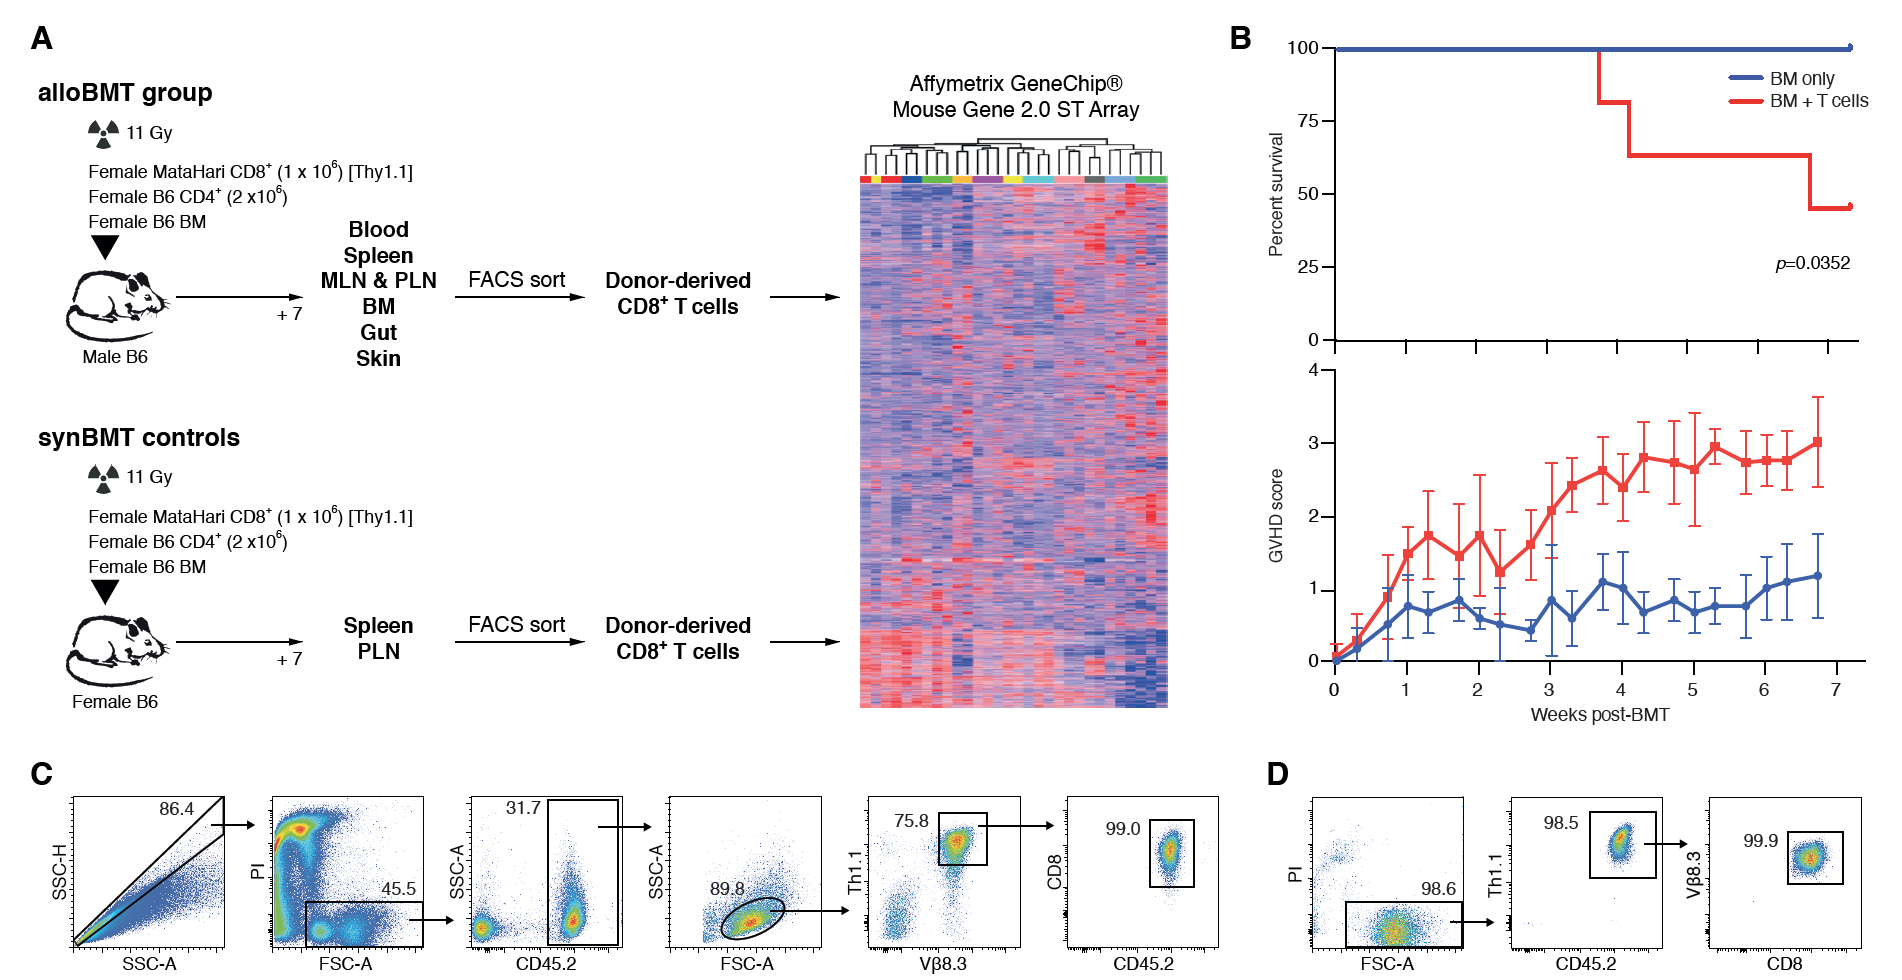
\includegraphics[width=0.9\textwidth]{Figures/Chapter1/MataHari.png}
   \caption{\small{\textbf{(A) Experimental setup.} Female MataHari CD8$\textsuperscript{+}$ T cells were transferred together with female B6 bone marrow and CD4+ T cells into lethally irradiated male B6 recipients (alloBMT group) or female B6 recipients (synBMT controls). Tissue harvesting took place at day +7 post-transplant and donor CD8$\textsuperscript{+}$ T cells were isolated and FACS sorted to high purity. Gene expression profile of sorted cells was assessed by whole-transcriptome microarray analysis. \textbf{(B) Characterization of the GVHD model.} Top graph: Kaplan Meier survival curve (log-rank Mantel-Cox test). Bottom graph: clinical GVHD score over time (mean ± SD). BM only (n=6), BM + T cells (n=11). \textbf{(C) Gating strategy used to sort donor derived CD8$\textsuperscript{+}$ T cells} (exclusion of doublets $\to$ exclusion of propidium iodide positive cells $\to$ exclusion of stroma cells $\to$ morphologic lymphocyte selection $\to$ selection of donor CD8$\textsuperscript{+}$ T cells based on the expression of congenic markers $\to$ confirmation of CD8 positivity). \textbf{(D) Gating strategy to evaluate purity at the end of each sort.} Abbreviations: BM, bone marrow; MLN, mesenteric lymph nodes; PLN, peripheral lymph nodes.} }
    \label{fig:1}
\end{figure}

\subsection{B6 into 129sv model}

\begin{figure}[H] 
    \centering
    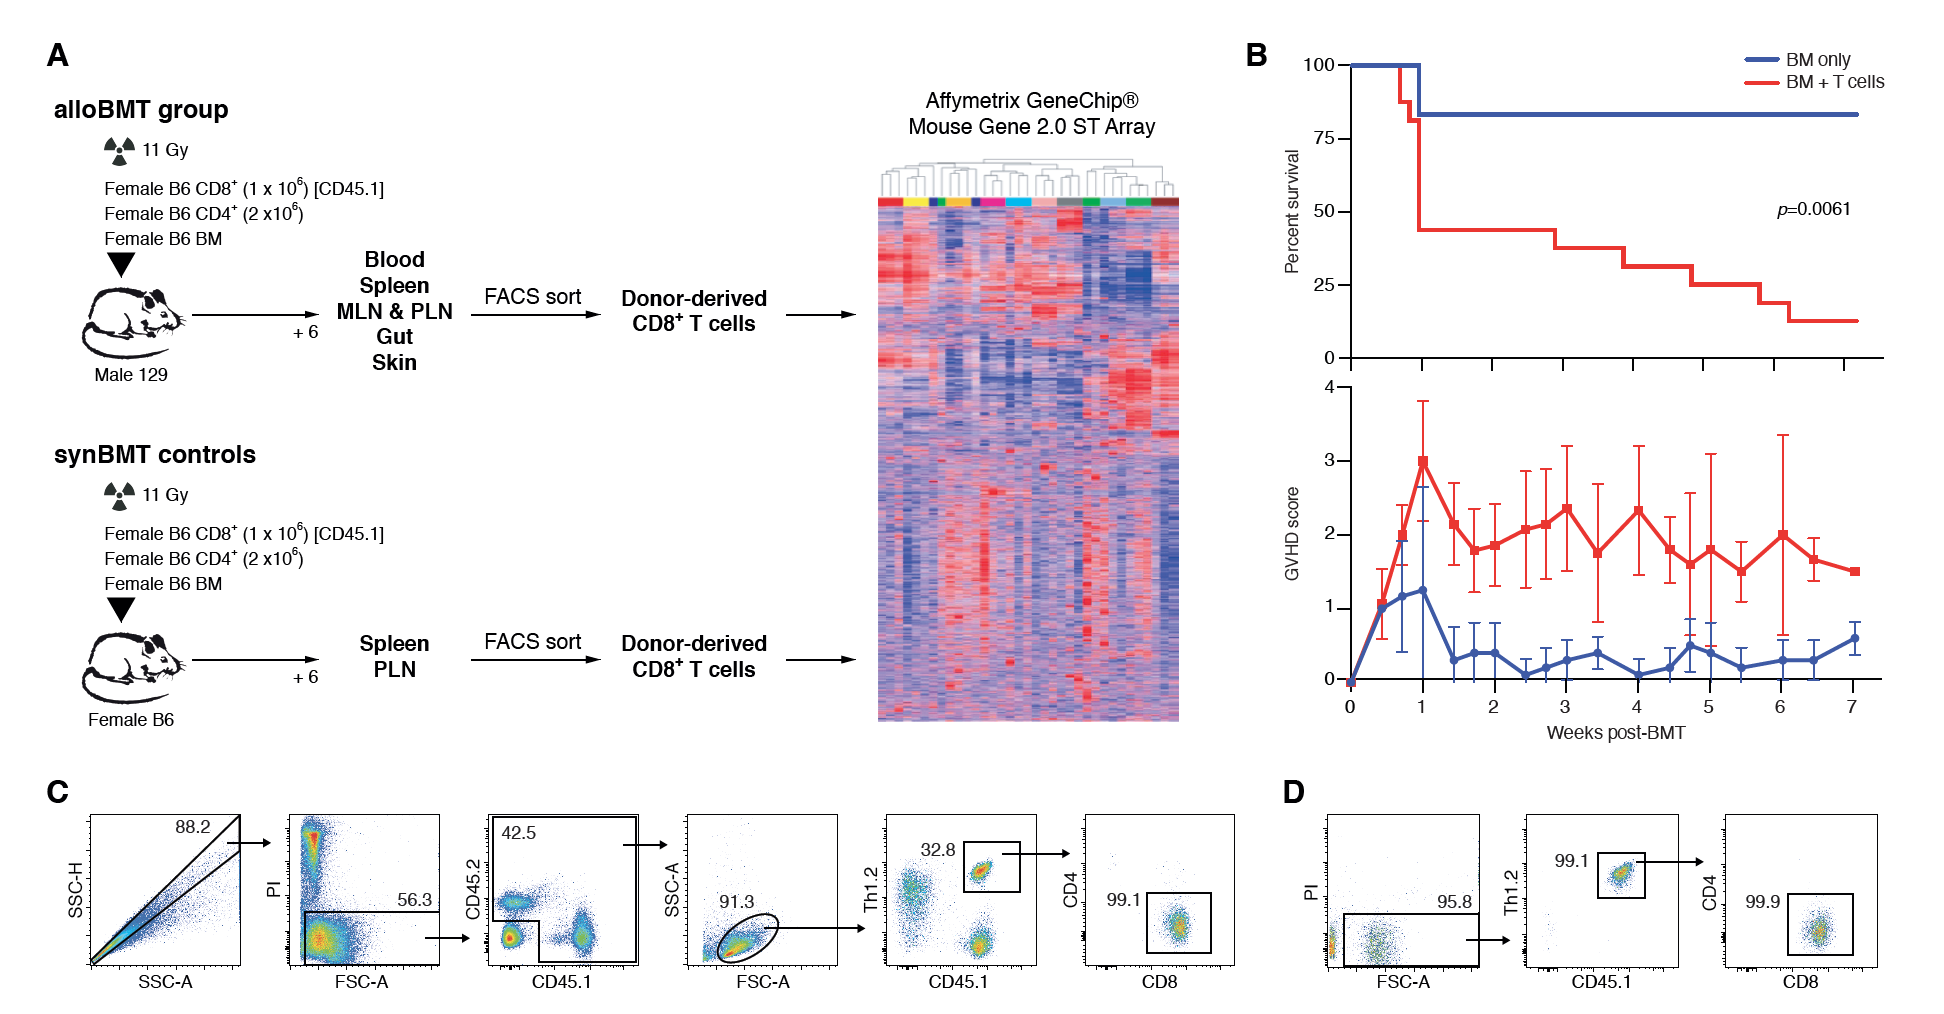
\includegraphics[width=0.9\textwidth]{Figures/Chapter1/B6_129.png}
   \caption{\small{\textbf{(A) Experimental setup.} Female B6 bone marrow and T cells were transferred into lethally irradiated male 129/Sv recipients (alloBMT group) or female B6 recipients (synBMT controls). Tissues were harvested at day +6 post-transplant and donor CD8$\textsuperscript{+}$ T cells were isolated and FACS sorted to high purity. Gene expression profiles of sorted cells was assessed by whole-transcriptome microarray analysis. \textbf{(B) Characterization of the GVHD model.} Top graph: Kaplan Meier survival curve (log-rank Mantel-Cox test). Bottom graph: clinical GVHD score over time (mean ± SD). BM only (n=6), BM + T cells (n=16). \textbf{(C) Gating strategy used to sort donor-derived CD8$\textsuperscript{+}$ T cells} (exclusion of doublets $\to$ exclusion of propidium iodide positive cells $\to$ exclusion of stroma cells $\to$ morphologic lymphocyte selection $\to$ selection of donor CD8$\textsuperscript{+}$ T cells based on the expression of congenic markers $\to$ confirmation of CD8 positivity). \textbf{(D) Gating strategy to evaluate purity at the end of each sort.} Abbreviations: BM, bone marrow; MLN, mesenteric lymph nodes; PLN, peripheral lymph nodes.} }
    \label{fig:2}
\end{figure}


\section{Systems biology approach}

Systems biology is perhaps best described as the adoption of a holistic approach to the task of understanding and interpreting complex biological systems. This field is based upon the premise that the whole is greater than the sum of the parts. In this context, "the whole" is often thought of as the networks that together from the living organism in its entirety. By it very nature this approach requires contribution from many scientific disciplines including biology, physics, computer science and bioinformatics to facilitate the exploration of new dimensions of data space and to tackle ever more challenging biological questions. 

As visualised in Figure 1.3, systems biology is usually thought of as a cyclical concept whereby new biological insights prompt the development of new, more powerful technologies to acquire increasing detailed data, which in turn necessitates the evolution of more advanced computational tools for appropriate analysis of the data obtained. Amongst other achievements, the ability to design predictive, multi-scale models now enables discovery of new biomarkers for disease, drug targeting as well as patient stratification based on unique genetic profiles.

\begin{figure}[H] 
    \centering
   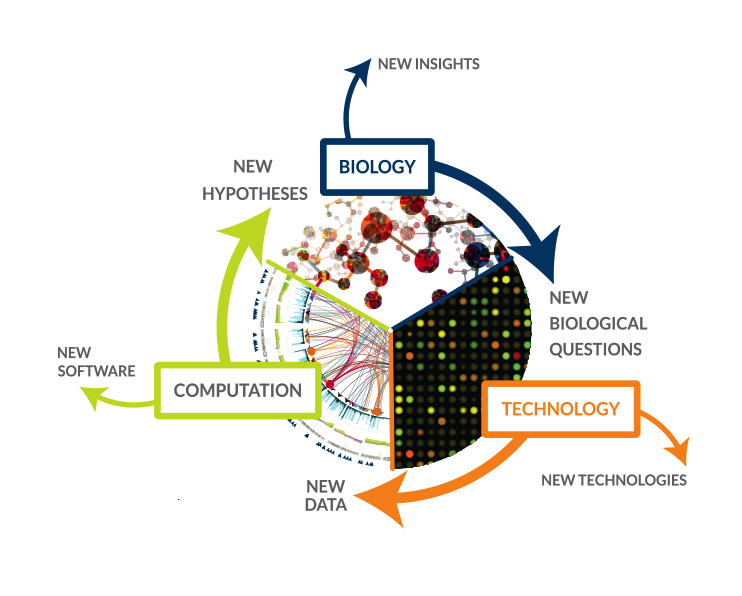
\includegraphics[width=0.8\textwidth]{Figures/Chapter1/systems_bio.jpg}
\caption{\small{The Institute for Systems Biology's depiction of how a cross-disciplinary environment allows for the establishment of a cycle where biology drives technology which in turn drives computation and so on.} }
    \label{fig:3}
\end{figure}

The high-throughput technologies in use today usually generate large lists of hundreds or thousands of potentially biologically interesting genes, but their biological interpretation is still a difficult task ~\autocite{Hua2009}. Indeed, there now exists a plethora of bioinformatics analytical/enrichment tools suitable for use with one or more of the currently available data types. Whilst this has undoubtedly been of huge benefit to thousands of research groups, the amount of choice can leave potential confused and overwhelmed regarding which is the best resource to meet their analytical requirements. It is often advisable for researchers to apply multiple tools from the same branch of analysis type to a given dataset and then manually compare the results and determine which offers the most biologically relevant insights ~\autocite{Hua2009}. In 2009, Huang \textit{et al.} performed a comprehensive analysis of the then available bioinformatics tools ~\autocite{Hua2009}. Although their list is now naturally very outdated, their classification of resources into three groups, namely singular enrichment analysis (SEA); gene set enrichment analysis (GSEA); and modular enrichment analysis (MEA), is still a valid separation. Briefly, SEA involves taking a pre-defined list of interesting genes, e.g. those found to be differentially expressed between case and control with a minimum 1.5 fold change, and linearly testing the enrichment of each known annotation term one-by-one. The major downsides of tools within this set are that the utility of the enrichment is heavily impacted by the quality of the pre-defined gene list and the output is often very large and not user-friendly. GSEA has a similar concept to SEA but with the key difference that GSEA takes as input all genes from a microarray experiment without pre-selection of significant genes. This naturally reduces the likelihood of analytical bias caused by prior determination of which genes are "interesting" and also means that even genes with seemingly small, but nonetheless interesting, changes in expression can still contribute to the analysis. Finally, MEA inherits the basic enrichment calculation found in SEA, but also incorporates network discovery algorithms by considering the term-to-term relationships. When considered together, these inter-relationships between enrichment terms may be of particular interest for the hypothesis under investigation and hence MEA will often produce results that are more easily related back to actual biological interactions than is the case for SEA or GSEA ~\autocite{Hua2009}.

As outlined in a previous section, our laboratory has generated two GVHD datasets using the B6 into 129sv and MataHari mouse models. Given the size and probable complexity of the microarray data obtained, we decided to utilise systems biology techniques to analyse these results and to try to identity clinically relevant gene modules that may help shed some light on the molecular pathways involved in the initiation and progression of GVHD in these mice. 

\subsection{Motivations: Benefit of clustering genes into modules?}

Virtually all cellular functions arise, at least on a fundamental level, as a direct consequence of gene expression patterns and subsequent protein-protein interactions. When considered at a more general level, these interactions can be seen to be organised into molecular pathways and feedback loops which together maintain homoeostatic functionality. Genes and the proteins they encode do not act in isolation but rather as part of one or more pathways or networks and hence it seems appropriate to analyse them in this context. Interconnected genes that form all or part of a biological network where nodes represent genes and edges the interactions between them, are often described as a gene module and it is these entitles that many bioinformatics tools try to identify by clustering together genes exhibiting similar patterns of expression ~\autocite{Lys2011}. These algorithms can be divided into many types based upon the mathematical premises they employ and include topology networks, network clustering, matrix decomposition and heuristic searches ~\autocite{Li2015}.

By attempting to identify gene modules within an expression dataset, we are far more likely to be in a position to understand the molecular implications of the condition/variable we are interested in than if we were to examine single, or even several genes, alone. However, this statement only holds true if the modules we identify and analyse are biologically meaningful and if one considers for a moment the detailed complexity of biological systems on every level, it can be seen that finding such modules is not as straightforward as it may initially appear. 

Many of the clustering algorithms developed to date group genes based on correlation networks between expression profiles as measured by microarray, or similar, techniques. These quantitative analyses typically produce measurements which can be described by an \textit{n} by \textit{m} matrix as follows: 

\begin{equation}
X = |x_ {il}|
\end{equation}

where the row indices correspond to network nodes (\textit{i} = \textit{1, 2,... n}) and the column indices (\textit{l} = \textit{1, 2,.. m}) correspond to sample measurements ~\autocite{Lan2008}. This can be written in the form:

\begin{equation}
\mathbf{X = |x_ {ij}|} = \left(
\begin{array}{c}
x_\textit{1} \\
x_\textit{2} \\
\vdots \\
x_\textit{n}
\end{array} \right)
\end{equation}

We refer to the \textit{i}-th row $x_i$ as the \textit{i}-th node profile across \textit{m} sample measurements. 

The rationale behind correlation network methodology, which is a common analytical choice among biologists, is to use network language to describe the pairwise relationships (correlations) between the rows of X ~\autocite{Lan2008}.

\subsection{How to evaluate quality of clustering results}

With advances in the development of stable gene clustering algorithms, researchers are now faced with questions of how to evaluate the accuracy and validity of modules they identify. However, given the prevalence of such algorithms, there are still surprisingly few established methods for the validation and evaluation of module gene sets. Until fairly recently, aside from size-limited experimental techniques to verify interactions between module members, studies largely relied upon function enrichment tools e.g. Gene Ontology (GO) and KEGG to determine the quality of their modules through enrichment. However, this method rarely produces evenly annotated modules and should theoretically be periodically re-analysed to account for updates made to the annotation database itself ~\autocite{Li2015}. 

In response to these shortcomings, research focus is now shifting to incorporate computational methods into the standard module validation analysis protocols. Such techniques often involve the probing of a modules architectural properties and collectively are sometimes known as Computational Validation Approaches based on Modular Architecture (CVAMA). CVAMA are suitable for application to modules of any size and are not reliant on external databases. In their recent review Li \textit{et al.} divided available CVAMA methods into topology-based approaches (TBA) and statistics-based approaches (SBA) and in the following brief summary we echo their distinctions ~\autocite{Li2015}. 

\subsubsection{topology-based approaches (TBA)}

A gene module can be seen as possessing several network topological features which can be used to quantify its physical parameters. Most analytical projects will tend to focus on one or several of these criteria which are deemed by the researchers to be most relevant for the purpose of establishing whether the proposed modules possess a non-random structure ~\autocite{Don2012}. Here we provide a list of typical parameters examined together with their definitions which have been taken from review of this topic by Doncheva \textit{et al.}~\autocite{Don2012}:

\paragraph{Connected components -} 
When considering an undirected network, any two given nodes are said to be connected if there are one or more edges between them. This parameter provides an indication of global connectivity, with a low value suggesting a strongly connected network.

\paragraph{Degree distributions -} 
For undirected networks, the node degree of a node \textit{n} is the number of edges to which it is linked. The \underline{node degree distribution} gives the number of nodes with degree \textit{k} for \textit{k = 0, 1, etc.} Nodes with high values of \textit{k} are known as hubs. In directed networks, the "in-degree" of node \textit{n} is the number of incoming edges and the "out-degree" is the number of outgoing edges. A network is termed scale-free if its degree distribution approximates a power law $k^{-\alpha}$ with the degree exponent \textalpha. As a general rule for biological studies, hubs with $\alpha >$ 3 are classed as irrelevant, those where 3 $< \alpha >$ 2 tend to possess hierarchical organisation and when $\alpha =$ 2 a 'hub-and-spoke' model (referring to the connectivity of the largest hub) is often seen. In the case of biological networks $\alpha$ is commonly between 2 and 3.

\paragraph{Neighbourhood-related parameters -} 
The set of neighbours for a particular node \textit{n} comprises its neighbourhood. The \underline{connectivity} \textit{kn} is the size of the neighbourhood of \textit{n} and the average of one can give an approximation of the average of the other. A networks density is a normalised version of this parameter. A network without any edges will have a density of 1, while the value for a clique will be 1.

\paragraph{Neighbourhood Connectivity} 

As mentioned above, the \underline{connectivity} of a node \textit{n} is the number of its neighbours. As such the neighbourhood connectivity of node \textit{n} is defined as the average connectivity of all neighbours of \textit{n}. The corresponding \underline{neighbourhood connectivity distribution} summarises the average of the neighbourhood connectivities of all nodes \textit{n} with \textit{k} neighbours for \textit{k = 0, 1, etc.} For directed networks, any given node possess three types of neighbourhood connectivity:

\begin{itemize}
    \item \emph{Only in }- the average out-connectivity of all in-neighbours of \textit{n}
    \item \emph{Only out }- the average in-connectivity of all out-neighbours of \textit{n}
    \item \emph{In and out} - the average connectivity of all neighbours of \textit{n}, where edge direction is ignored
\end{itemize}

Based on these definitions there are three equivalently named neighbourhood connectivity distributions.

\paragraph{Shortest paths -}

The length of a path is represented by the number of edges forming it. The length of the shortest path, or distance, between two nodes \textit{n} and \textit{m} is denoted by L(\textit{n,m}). The \underline{shortest path length distribution} gives the number of node pairs (\textit{n,m}) with L(\textit{n,m}) = \textit{k} for \textit{k = 0, 1, etc.} The \underline{eccentricity} of a node \textit{n} is the maximum non-infinite length of a shortest path between \textit{n} and another node in the network. The \underline{network diameter} is the maximum node eccentricity. 

the \underline{network radius} is defined as the minimum of the nonzero eccentricities of the nodes in the network. The \underline{average shortest path length} gives the expected distance between two connected nodes.

\paragraph{clustering coefficients -}

In undirected networks, the clustering coefficient $C_n$ of a node \textit{n} is defined as $C_n = 2e_n/(k_n(k_n–1))$, where $k_n$ is the number of neighbours of \textit{n} and $e_n$ denotes the number of edges between all neighbours of \textit{n}. In directed networks, this coefficient is parametrised by $C_n = e_n/(k_n(k_n–1))$. 

In both instances, the clustering coefficient is a ratio \textit{N/M}, where \textit{N} is the number of edges between the neighbours of \textit{n}, and \textit{M} the maximum number of edges that could possibly exist between the neighbours of \textit{n}. For any given node \textit{n}, this value is always between 0 and 1. 

The \underline{network clustering coefficient} is the average of the clustering coefficients of all nodes in the network and the \underline{average clustering coefficient distribution} gives the average of the clustering coefficients for all nodes \textit{n} with k neighbours for \textit{k = 2, 3, etc}.  

\paragraph{Shared neighbours -}

Defined as \textit{P}(\textit{n,m}), this parameter represents the number of interaction partners shared between nodes \textit{n} and \textit{m}. The \underline{shared neighbours distribution} gives the number of node pairs (\textit{n,m}) with \textit{P}(\textit{n,m}) = \textit{k} for \textit{k = 1, 2, etc}. 

\paragraph{Topological coefficients -}

The topological coefficient $\textit{T}_n$ of a node \textit{n} with $\textit{k}_n$ neighbours is computed as: 

\begin{equation}
\textit{k}_n = avg (\textit{J}(\textit{n, m}))/\textit{k}_n
\end{equation}

Here \textit{J}(\textit{n, m}) is defined for all nodes \textit{m} that share at least one neighbour with \textit{n}. 
The value \textit{J}(\textit{n, m}) is the number of neighbours shared between the nodes \textit{n} and \textit{m}, plus 1 if there is an edge between \textit{n} and \textit{m}. This coefficient is a relative measure for the extent to which a given node \textit{n} shares neighbours with other nodes. 

\paragraph{Stress centrality -}

The stress centrality of a given node \textit{n} is the number of shortest paths passing through \textit{n}. The \underline{stress centrality distribution} gives the number of nodes with stress \textit{s} for \textit{s = 1, 2, etc}. 

\paragraph{Betweenness centrality -}

The betweenness centrality $C_b\textit{(n)}$ of a node \textit{n} is defined as:

\begin{equation}
C_b\textit{(n)} = \textstyle \sum_{s\neq n\neq t}^{}  (\sigma_{st}(n)/\sigma_{st})
\end{equation}

where, \textit{s} and \textit{t} are nodes in the network other than \textit{n}, $\sigma_{st}$ gives the number of shortest paths from \textit{s} to \textit{t}, and $\sigma_{st}(n)$ is the number of shortest paths from \textit{s} to \textit{t} that pass through \textit{n}.

This parameter is only computed when a network is comprised of single edges alone. 

The betweenness value for each node \textit{n} is normalised to lie between 0 and 1 by dividing the number of node pairs excluding \textit{n} as follows:
\begin{equation}
(\textit{N} -– 1)(\textit{N} -– 2) / 2
\end{equation}
 where \textit{N} is the total number of nodes in the connected component that \textit{n} belongs to. The betweenness centrality of a node reflects the amount of control it exerts over the interactions of other nodes in the network.

\paragraph{Closeness centrality -}

The closeness centrality $C_\textit{(n)}$ of a node n is the reciprocal of the average shortest path length. The closeness centrality of each node \textit{n} is a value between 0 and 1 and is a measure of how quickly information spreads from a given node \textit{n} to other reachable nodes in the network.

Several topological indexes have also been developed to evaluate a given module's likely validity. These include the the network perplexity index of Entropy where a good quality module is expected to have a low entropy ~\autocite{Zha2009}. This index is typically defined as follows: 

\begin{equation}
Entropy (M) = -\textstyle \sum_{J \in {bins}}^{} P_j log_2 P_j
\end{equation}

Another widely used single index is the NB Value which is used to identify modules with high intra-modular connectivity (NB $\geq$ 0.5) ~\autocite{Oza2010}. The NB Value represents a ratio of edges within a module and the total number of edges between modules:

\begin{equation}
NB = \frac{\sum e(i)} {\sum d(i)} 
\end{equation}

To be of informative value it is vital that the index chosen to validate a module should be independent of the methods used to identify the module. It is also common practice for multiple topological indexes or module preservation statistics to be combined into an integrated measure for the overall assessment of module validity or preservation. Perhaps the most widespread composite preservation statistic used to validate whether a module is significantly preserved in another network is the Z\textsubscript{summary} score ~\autocite{Lan2011}: 

\begin{equation}
Z_{summary} = \frac{Z_{density} + Z_{connectivity}} {2} 
\end{equation}

A Z\textsubscript{summary} score of $\geq$ 10 indicates that a module is strongly preserved, a value between 2 and 10 suggests moderate preservation and if this index produces a score $\leq$ 2 then no preservation is found. 

\subsubsection{statistics-based approaches (SBA)}

As well as exhibiting some form of modular structure which can be analysed using the topological criteria detailed above, a "good" gene module should be statistically significant i.e. its architecture distribution ought to be very unlikely to be obtained by chance in a randomised network. It is often also important to quantify relationships between modules and phenotypic characteristics and this too requires some measurement of statistical significance. Depending on the biological context it is possible to use binary or mixed integer linear models to validate causal or dependent relationships between network modules and biological phenotypes ~\autocite{Hen2011,Sch2011,Shi2010}. Using a permutation test with a \textit{p}-value calculated by estimating the null distribution we are able to determine whether the composition of a given module is higher than expected by chance or is associated with a particular disease phenotype ~\autocite{Jia2012}. As mentioned above, comparative network analysis techniques such as Z\textsubscript{summary} can also aid the identification of conserved modules across networks or species, as well as providing insight into the reproducibility of the module in question. 


\subsection{Two complementary approaches to module definition}

\subsection{Prior generation of MataHari modules using WGCNA}

To tackle the hypothesis mentioned previously, i.e. to measure the respective roles of lymphoid organs and peripheral tissues in dictating T cell effector programs that result in tissue injury, our team began by characterising the transcriptional response of donor CD8$\textsuperscript{+}$ effector T cells as they trafficked to multiple sites during the evolution of GVHD. This enabled the analysis of how T cells differentiate within secondary lymphoid organs (SLO) compared to those in peripheral tissues. Experiments using the MataHari and B6 into 129sv GVHD models were performed as outlined in Figures 1.1 and 1.2 respectively. Once microarray data had been acquired from the B6 into 129sv experiments, skin- and gut-tissue specific genes, determined using PaGenBase, were removed from the datasets to correct for any contamination by other celltypes. Multi-dimensional scaling (MDS) was performed on both datasets and as evidenced by Figure 1.4A, not only do allogeneic recipients segregate separately from both na\"ïve T cells and those undergoing proliferation within lymphatic tissues, but there is also a clear distinction within recipients of allogeneic BMT between those T cells deriving from secondary lymphoid organs (plotted as blue circles) and those within GVHD target tissues (shown as red circles in the plot). 

\begin{figure}[H] 
    \centering
   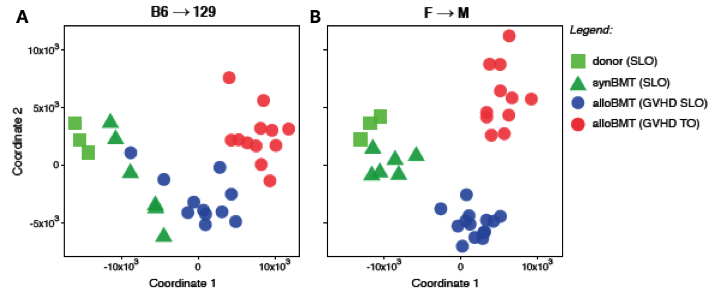
\includegraphics[width=0.8\textwidth]{Figures/Chapter1/lab_MDS_plot.png}
\caption{\small{Multi-dimensional scaling (MDS) plots depicting the proximity of the transcriptional profiles of donor derived CD8$\textsuperscript{+}$ T cells isolated from the spleen, lymph nodes, blood, gut and skin, in the two model systems (B6 into 129sv and MataHari Female $\to$ Male).} }
    \label{fig:4}
\end{figure}

It was concluded that these observed differences in gene expression profiles could be the result of either tissue environment-dependent re-programming or the selection of pre-existing variants from the bulk population. To exclude the latter option the experiments were repeated in the MataHari B6 female $\to$ B6 male. This BMT model involves the transfer of na\"ive MataHari CD8$\textsuperscript{+}$ T cells transgenic for a TCR that recognises a single, ubiquitous HY antigen, Db-Uty. As can be seen in Figure 1.4B, the expression profiles of T cells found in GVHD target organs are again clustered away from those in the secondary lymphoid organs. Additionally, there was a substantial amount of overlap identified between effector T cell expression profiles from each tissue in the MataHari Female $\to$ Male dataset and the equivalent sample in the B6 into 129sv model which supports the theory that differences in effector T cell profiles reflected the source tissue and were independent of the T cell receptor repertoire. Given the profound separation seen between tissue groups in the MataHari Female $\to$ Male model, this dataset was taken forward for further analysis. 

Using the analytical method Weighted Gene Correlation Network Analysis (WGCNA), which is detailed in Chapter \ref{Chapter3}, modules of co-expressed genes were identified within the Female $\to$ Male data in the hope that they may assist in gaining an understanding how tissue specific effector T cell transcriptional programs develop. A total of 31 such gene modules were found and the inter-module expression patterns were seen to vary substantially between both the type of BMT (syngeneic or allogeneic) and the tissue source of the T cells. This diversity in module expression profiles, which is portrayed in Figure 1.5A, even extended to tissue sub-compartments (e.g. the dermis versus the epidermis). As evidenced by this Figure, a marked distinction was observed between those modules up-regulated in GVHD target organs compared to the secondary lymphoid organs which is of great interest given our hypothesis of tissue specific re-programming of effector T cells. In order to determine how well these 31 modules were conserved in the B6 into 129sv model the Z\textsubscript{sum} composite preservation measurement was used. Of the 31 modules identified in the Female $\to$ Male dataset 30 were found to be conserved in the B6 into 129sv dataset based on a Z\textsubscript{sum} > 2.0, while 19 modules passed the cut-off at Z\textsubscript{sum} > 10. These 19 modules were subsequently annotated to identify enriched biological processes using the Gene Ontology database ~\autocite{Ash2000,GO2015} and candidate driver genes i.e. genes exhibiting high intra-modular connectivity were pinpointed. The most significant biological process annotations and likely driver genes are shown in Figure 1.5B. 

\begin{figure}[H] 
    \centering
   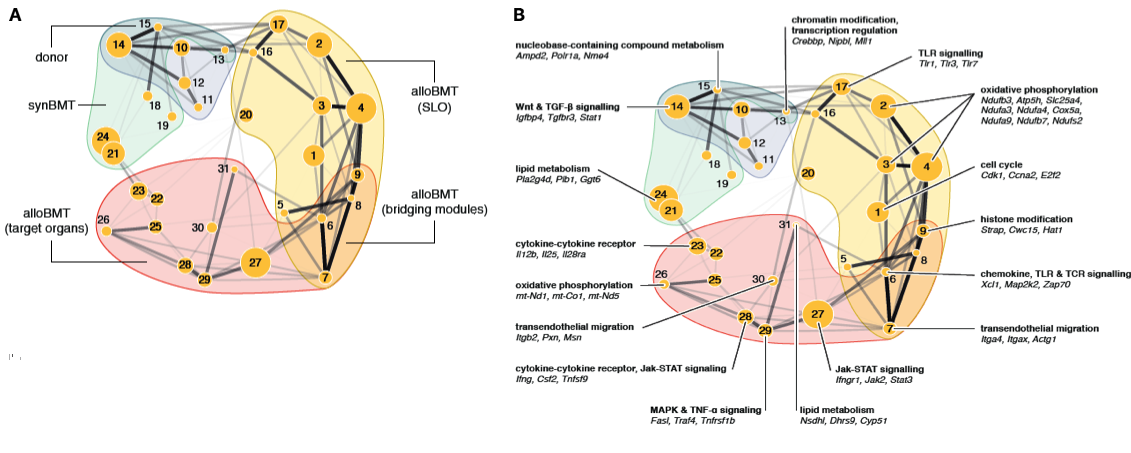
\includegraphics[width=0.9\textwidth]{Figures/Chapter1/MH_mods.png}
\caption{\small{A. Summary Eigengene network where shaded areas represent MataHari Female $\to$ Male module clusters associated with the surveyed experimental groups and GVHD subgroups. B. MataHari Female $\to$ Male modules classified according to the main classes of Gene Ontology terms of the annotated genes. Putative driver genes for each conserved module were identified on the basis of high intra-modular connectivity (3 examples per module).} }
    \label{fig:5}
\end{figure}

Further details and discussions of these findings will not be included here but given the importance of this dataset for work presented later in this report, the following represents a summary of the authors primary observations: 

\begin{enumerate}
    \item Several, strongly interconnected gene clusters segregated primarily with the SLO origin of effector T cells e.g. M17 was strongly correlated with T cells from the LN but negatively correlated with those of GVHD target organs; 
    \item M1 which contains genes associated with DNA replication and the cell cycle mapped to blood and BM-derived effector T cells;
    \item M3 segregated with the spleen and BM TE and was almost exclusively comprised of fatty acid oxidation and oxidative phosphorylation related genes;
    \item M7 which contained genes encoding proteins implicated in cytoskeletal reorganisation and transendothelial migration was the most densely interconnected of the bridging modules;
    \item  The largest GVHD target organ-specific module was M27. This module was enriched for multiple intracellular signalling gene pathways including MAPK and JAK-STAT;
    \item M28 was highly specific for effector T cells of the epidermis and contained a strong Ifng-related signal with genes for multiple pro-inflammatory cytokines, cytokine receptors and downstream adaptors;
    \item  M29 segregated with the majority of GVHD target organs and is considered by the authors to represent a pan-GVHD target organ gene cluster;
    \item  Driver genes identified within the M7, M28 and M29 modules, showed a high degree of overlap with a Th1/17-related pathogenicity gene cluster that is linked to aggressive T cell autoimmunity
\end{enumerate}
 
It can thus be seen that this MataHari dataset together with the WGCNA-derived gene modules discussed briefly above represent a highly useful and detailed resource from which we can potentially learn much regarding the impact of tissue specific effector T cell imprinting on GVHD pathology. 
 
